\section{Projektplan}

\subsubsection*{Zweck dieses Dokuments}
Dieses Dokument beschreibt den Projektplan des Projekts «Solution Strategy mit der Methode 635 als Cross Plattform App». Es beinhaltet die Planung, die Organisation sowie weitere Aspekte und liefert damit eine Übersicht über das Projekt. Es dient daher als Grundlage für den Verlauf des Projekts.

\subsubsection*{Gültigkeitsbereich}
Der Gültigkeitsbereich erstreckt sich über die gesamte Dauer des Projekts. Der Zeitraum geht vom 18. Februar 2019 bis zum 14. Juni 2019. Das Projekt findet im Rahmen des Moduls «Bachelorarbeit» im Frühlingssemester 2019 statt.

\subsubsection*{Verweise}
An dieser Stelle ist noch zu anzumerken, dass einzelne Textstellen von eigenen, älteren Projektplänen verwendet wurden. Dabei handelt es sich um Projektpläne von Engineering-Projekten oder Studienarbeiten.

Im Speziellen zu erwähnen ist die Tatsache, dass dieser Bachelorarbeit eine Studienarbeit («Methode 635 als Cross Plattform App mit Xamarin») vorherging. Es kann daher sein, dass in einigen Textstellen auf diese Studienarbeit verwiesen wird. 

\subsection{Projektziel}
Die papiergestützte Methode 635 ist eine Kreativitäts- und Brainwriting-Technik, für die es bisher noch keine Unterstützung in mobilen Apps gab. Eine Studienarbeit im Herbstsemester 2018/2019 konzipierte und implementierte daher einen ersten Prototyp einer SmartPhone App für die Methode 635; Cross Platform Support (Android- und iOS) wurde durch Verwendung von Xamarin erreicht. Ein Vorteil einer derartigen mobilen Anwendung ist, dass Anwender die Methode 635 nutzen können, wenn sie sich nicht ständig an einem Ort befinden.
 
In dieser Bachelorarbeit sollen weitere Features implementiert werden auf Basis der Testergebnisse für den bestehenden Prototypen. Im Fokus steht dabei insbesondere die Software Engineering Aktivität "Solution Strategy" aus dem Buch „Effektive Softwarearchitekturen“ von G. Starke, die in der HSR-Vorlesung Application Architecture behandelt wird.

Mehr zum Thema Projektziel ist dem Anhang \ref{sec:aufgabenstellung} zu entnehmen.

\subsubsection*{Einschränkungen}
Dieses Projekt ist auf die Dauer des Frühlingssemesters 2019 begrenzt (bis 14. Juni 2019). Der Gesamtaufwand für diese Arbeit sollte 360 Arbeitsstunden pro Person (gesamthaft 720 Stunden) nicht übersteigen. Bleibt am Ende Zeit übrig, werden optionale Features implementiert.

\subsection{Projektorganisation}
In unserem Projekt arbeiten wir in einer flachen Organisationsstruktur, wobei die wesentlichen Entscheide im ganzen Projektteam und/oder mit dem Dozenten an den wöchentlichen Besprechungen getroffen werden. An den Besprechungen getroffene Entscheidungen werden in Protokollen dokumentiert. Die Projektmitglieder sind innerhalb des Teams gleichgestellt.

\subsubsection*{Organisationsstruktur}
Die Projektmitglieder sowie deren Verantwortung sind der Abbildung \ref{fig:organisation} zu entnehmen.
\begin{figure}[h]
	\centering
	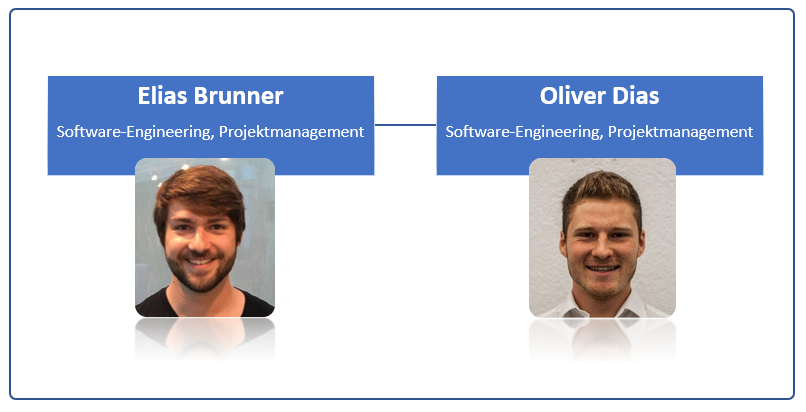
\includegraphics[width=1\linewidth]{img/projekt-plan/organisation}
	\caption[Organisation Methode 635]{Methode 635 Organisation}
	\label{fig:organisation}
\end{figure}


\subsubsection*{Ansprechspartner}
Da diese Arbeit eine Weiterführung der Studienarbeit darstellt, bleibt der bisherige Ansprechpartner bestehen.

\begin{description}[leftmargin=!,labelwidth=\widthof{\bfseries Betreuer}]
	\item[Betreuer] Prof. Dr. Olaf Zimmermann ist der betreuende Dozent für diese Bachelorarbeit. Er ist neben der Betreuung auch für die Bewertung des Projekts verantwortlich. 
\end{description}

\subsection{Projektmanagement}
Eine ausführliche Iterationsplanung mit den dazugehörigen Meilensteinen befindet sich auf \href{https://hsr-ba.atlassian.net/}{Jira}. Die aufgewendeten Zeiten für ein Issue werden ebenfalls dort erfasst.



\subsubsection*{Dokumentenplan}
Wie das Projekt selbst, werden auch sämtliche Dokumente ständig überarbeitet und angepasst. Grundsätzlich umfasst der Dokumentenplan aber folgende Bestandteile:

\begin{description}[leftmargin=!,labelwidth=\widthof{\bfseries Architekturdokumentation}]
	\item[Projektplan] Der Projektplan umfasst den groben Ablauf des Projektes und legt unter anderem das Vorgehen bei der Entwicklung fest oder wie mit Risiken umgegangen wird.
	\item[Anforderungsspezifikation] In der Anforderungsspezifikation werden funktionale sowie nicht-funktionale Anforderungen definiert.
	\item[Architekturdokumentation] Hier wird dokumentiert wie die Architektur des gesamten Systems aufgebaut ist.
	\item[Architekturentscheide] Hier wird aufgezeigt warum wir uns für diese Architektur entschieden haben.
	\item[Installationsanleitung] In der Installationsanleitung wird gezeigt, wie die Applikation auf dem eigenen Smartphone installiert werden kann.
\end{description}
 

\subsubsection*{Besprechungen}
Das Projektteam trifft sich einmal in der Woche, um sich über den aktuellen Stand des Projekts auszutauschen, Fragen zu klären, Probleme anzugehen oder die nächsten Schritte zu planen. 

Diese wöchentlichen Besprechungen finden, falls nicht anders vorgesehen, jeden Dienstagmorgen um 09:00 Uhr statt. 

Über jede Besprechung wird Protokoll geführt. Dies mit dem Ziel, die Entscheidungen festzuhalten und Missverständnisse zu vermeiden.


\subsubsection*{Umgang mit Risiken}
Um auch auf unbekannte Risiken vorbereitet zu sein, ist am Ende des Projektes eine Reserve eingeplant. Zudem haben sich beide Teilnehmer bereit erklärt ihr Engagement punktuell zu erhöhen, falls die Situation dies erfordert. Diese Erhöhung sollte jedoch nur Phasenweise erfolgen und in einer folgenden Phase kompensiert werden. 

Die häufigsten Risiken wurden mit einer Risikotabelle (Unterkapitel \ref{risiko-tabelle}) be\-rück\-sichtigt, die aktuell gehalten wird und beim Planen miteinbezogen gezogen wird. 

\subsubsection*{Qualitätsmassnahmen}
Das Endprodukt dieses Projekts soll von möglichst hoher Qualität sein. Wie in Tabelle \ref{tab:Massnahmen} zu sehen ist, treffen wir folgende Massnahmen, um diese Qualität zu erreichen.

\renewcommand{\arraystretch}{2}
\begin{table}[h]
  \begin{tabular}{ | p{3cm} | c | p{5.5cm} | }
  	\hline
    \textbf{Massnahme}			& \textbf{Zeitraum}	 	& \textbf{Ziel} \\
    \hline
    Meeting im Team und mit Betreuer & Jede Woche & Projektstand aufzeigen, allfällige Probleme möglichst früh erkennen.\\
    \hline
    Code Reviews & Bei jedem Pull Request & Die Qualität des Codes wird durch die Einhaltung der Code Style Guidelines verbessert.\\
    \hline
  \end{tabular}
  \caption[Projektplan]{Massnahmen}
  \label{tab:Massnahmen}
\end{table}

\subsubsection*{Arbeitspakete}
Die gesamte Arbeit ist in Arbeitspakete unterteilt, die auf Jira verwaltet werden. Dabei sind relevante Informationen wie die Komplexität, Dauer, der damit verbundene Epic und die Unterteilung in Arbeitskategorie erfasst.

Für die Abschätzung der Komplexität der Arbeiten verwenden wir \textbf{Story Points}. Dabei einigen wir uns auf folgendes Schema:

\renewcommand{\arraystretch}{1.5}
\begin{table}[h]
	\centering
	\begin{tabular}{| l | r |}
		\hline
		\textbf{Story Points} & \textbf{Bedeutung}\\
		\hline
		1-3 & Niedrige Komplexität \\
		4-6 & Mittlere Komplexität \\
		7-9 & Komplexe bis sehr komplexe Arbeit\\
		\hline
	\end{tabular}
	\caption[Story-Points]{Story Points Komplexität}
	\label{tab:story-points}
\end{table}

Das Unterteilen in drei Punkte pro Komplexitätsgrad ermöglicht ein genaueres Abschätzen innerhalb des Komplexitätsgrades. Story Points können nicht direkt in zeitlichen Aufwand umgerechnet werden. Für den benötigten Zeitaufwand existiert ein separates Feld.

Um die Pakete logisch unterteilen zu können, existieren Arbeitskategorien. Diese werden mit Labels auf den Tickets markiert und können folgende Werte annehmen:
\begin{description}[leftmargin=!,labelwidth=\widthof{\bfseries ProjektManagement}]
	\item[ProjektManagement] Alle Aufgaben, die im Zusammenhang mit Projektmanagement stehen, zum Beispiel das Risikomanagement.
	\item[Planung] Planungsaufgaben. Zum Beispiel steht jede Woche ein Teammeeting an, welches dieser Kategorie zugeordnet ist.
	\item[Dokumentation] Arbeiten, welche für Dokumentation des Projektes gemacht werden.
	\item[Infrastruktur] Diejenigen Arbeitspakete, die für die Entwicklung und für den Betrieb des Projekts notwendig sind. Ein Beispiel dafür kann das Einrichten eines Codequalitätstools sein. 
	\item[Entwicklung] Arbeitspakete welche mit der Programmierung der Applikation in Zusammenhang stehen.
	\item[Testing] Arbeitspakete wie zum Beispiel das Schreiben von Testfällen kann dieser Arbeitskategorie zugewiesen werden.
	\item[Design] Hierzu zählen Arbeitspakete wie das Ausarbeiten von Benutzeroberflächen.
	\item[Analyse] Typische Analyseaufgaben ist zum Beispiel das Recherchieren für bestimmte Frameworks, Bibliotheken, etc. 
\end{description}

\subsubsection*{Eingesetzte Werkzeuge}
Um ein gutes Arbeiten zu ermöglichen, stehen viele Tools zur Verfügung, die im Folgenden beschrieben sind. Die primäre Entwicklungsumgebung ist Visual Studio und \href{https://visualstudio.microsoft.com/de/vs/mac/}{Visual Studio for Mac}.

\subsection{Entwicklung}
Der Entwicklungscode wird in öffentlichen Github Repositories unter der Organisation \textbf{BrainingOutOfBox} gehalten. Für alle einzelnen Teile des Projekts gibt es ein eigenes Repository.

\begin{description}[leftmargin=!,labelwidth=2cm]
\item [Doc] \href{https://github.com/BrainingOutOfBox/Doc-BA}{Dieses Repository} enthält alle relevanten Dateien, welche für die Dokumentation von Relevanz sind.
\item [App] \href{https://github.com/BrainingOutOfBox/App}{Dieses Repository} enthält den gesamten Code für die Xamarin Applikation.
\item [API] \href{https://github.com/BrainingOutOfBox/API}{Dieses Repository} enthält den gesamten Code für das Play-Backend.
\end{description}

\subsubsection*{Vorgehen bei der Entwicklung}
Jedes Teammitglied verfügt über eine lokale Kopie der Repositories von Github. Für jede Aufgabe/Issue wird ein eigener Branch erstellt. Darin werden die Änderungen für diese Aufgabe vorgenommen. Die Änderungen sollen mit sinnvollen und präzisen Commit-Notizen festgehalten werden. Um ein Tracking der Änderung möglichst effizient zu gestalten, gilt es möglichst früh, möglichst viel zu commiten.

\begin{quote}
	"Commit early and commit often"    
\end{quote}

Dies wurde uns so in den Modulen SE1 und SE2 vermittelt.
%Evtl. muss hier noch ein allgemeiner Workflow für das Arbeiten eingefügt werden.

\subsubsection*{Code Guidelines}
Da Xamarin auf .Net bzw. C\texttt{\#} aufbaut, werden die Code Guidelines von .Net verwendet. \cite{guidelines-DotNet}

\subsubsection*{Builden und testen der App}
Für das automatisierte Builden und Testen nach einem Commit wird auf \href{https://appcenter.ms/orgs/BrainingOutOfBox/apps/BrainingOutOfBox-App}{Visual Studio App Center} von Microsoft gesetzt. Zum einen ermöglicht es eine einfache Integration von GitHub und zum anderen bringt es alles mit, um Xamarin Apps automatisch zu builden, testen und deployen. 

\subsection{Zeitliche Planung}

\subsubsection*{Phasen}
In unserem Projekt verwenden wir die vier Phasen von Rational Unified Process (RUP) \cite{RUP} mit dem Zusatz einer Testing Phase, welche in RUP nicht vorgesehen ist. Innerhalb der einzelnen Phasen wenden wir allerdings das Konzept von SCRUM \cite{SCRUM} an.  
\begin{description}[leftmargin=!,labelwidth=\widthof{\bfseries Construction Phase}]
	\item [Inception Phase] In der Inception Phase geht es hauptsächlich darum, Jira einzurichten und den Projektplan zu schreiben. Diese Phase beinhaltet den Sprint Inception-1.
	\item [Elaboration Phase] Die Elaboration Phase umfasst den Sprint Elaboration-1. Hier werden die Anforderungen an die Applikation definiert, den Proof-of-Concept für die Skizzenfunktion durchgeführt und weitere konzeptionelle Arbeiten erledigt. Am Ende der Phase müssen alle konzeptionellen Fragen geklärt sein. 
	\item [Construction Phase] In der Phase der Construction geht es an die Umsetzung der Applikation. Hierfür sind 5 Sprints eingerechnet. Dafür stehen die Sprints Construction-0, Construction-1, Construction-2, Con\-struc\-tion-3, Construction-4 zur Verfügung.
	\item [Testing] In der Testing Phase bzw. im Sprint Testing-1 wird die gesamte Applikation einem User Test unterzogen.
	\item [Transition Phase] In der letzen Phase werden alle abzugebende Dokumente nochmals durchgelesen und allenfalls überarbeitet. Dies geschieht im Sprint Transition-1.
\end{description}

\subsubsection*{Sprints}
Ein einzelner Sprint dauert zwei Wochen. So stehen pro Woche insgesamt 48 Stunden für die Bachelorarbeit zur Verfügung. In unserem Projekt sind folgende Sprints geplant:

\begin{center}
	\begin{longtable}{| l | p{10cm} |}
		\hline
		\textbf{Sprint} & \textbf{Arbeiten}\\
		\hline
		\textit{Inception-1 } & 
			\begin{itemize}[noitemsep]
				\item Projektplan erstellen
				\item Jira einrichten
				\item einzelne Risikos einschätzen
			\end{itemize}\\
		\hline
		\textit{Elaboration-1 } & 
			\begin{itemize}[noitemsep]
				\item Vorstudie zu einzelnen Themen durchführen
				\item Domainmodell überarbeiten
				\item NFAs sowie FAs überarbeiten
				\item Mockups für zusätzlich benötigte Oberflächen zeichnen
				\item PoC für Skizzenfunktion erstellen
			\end{itemize}\\
		\hline
	\end{longtable}
\end{center}

\begin{landscape}
	\thispagestyle{empty}
	\label{subsec:timeline}
		\begin{figure}[h]
			\centering
			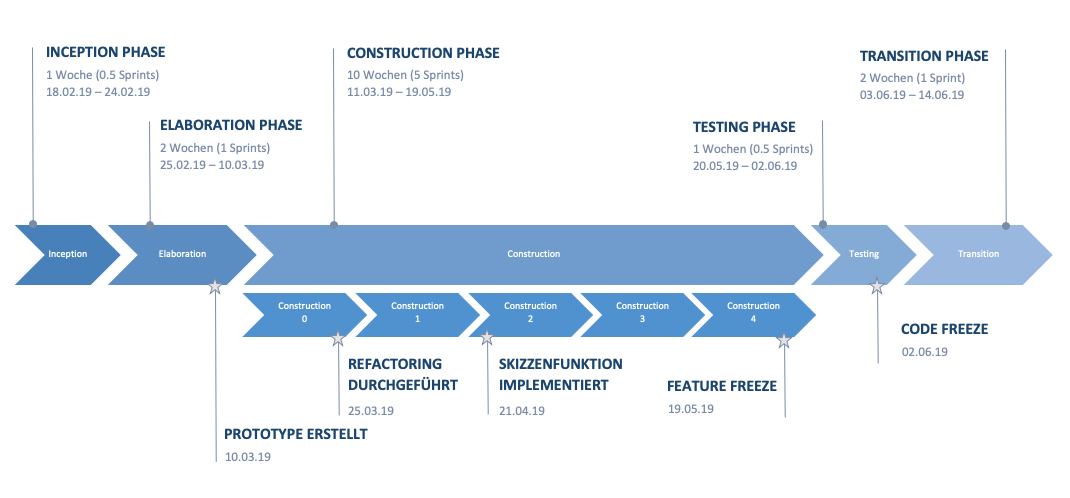
\includegraphics[width=1\linewidth, height=9.6cm]{img/projekt-plan/projekt-plan}
			\caption[Projektplan]{Projektplan}
			\label{fig:projekt-plan}
		\end{figure}
	\vspace{0.5cm}
	
\end{landscape}

%TODO:  Projektrisiken